\documentclass[11pt]{article}
%\documentclass[11pt]{amsart}
\usepackage{geometry}                % See geometry.pdf to learn the layout options. There are lots.
\geometry{letterpaper}                   % ... or a4paper or a5paper or ... 
%\geometry{landscape}                % Activate for for rotated page geometry
\usepackage[parfill]{parskip}    % Activate to begin paragraphs with an empty line rather than an indent
\usepackage{hyperref}
\usepackage{graphicx}
\usepackage{amsmath,amssymb,latexsym}
\usepackage{epstopdf}
\DeclareGraphicsRule{.tif}{png}{.png}{`convert #1 `dirname #1`/`basename #1 .tif`.png}

\title{RIFIDI Engineering}
\author{James Percent \\ james@pramari.com}
\date{10/10/2010}                                           % Activate to display a given date or no date

\begin{document}
\maketitle

\section{Introduction}

This document is the basis for the getting started on the RIFIDI engineering team.  It's the single source for all the information you need to get going.  It's obviously evolving, so let us know if you find anything missing, outdated, or incorrect.

\subsection{Operating System}\label{os}

This section provides information about installing and configuring Ubuntu Linux, which is our supported platform.  We should be able to run on any platform that supports Java 6, but such configurations are beyond the scope of this document.

The supported version of Ubuntu is 10.04.1 LTS, Lucid Lynx \cite{ubuntu, lucid}.  Instructions regarding Ubuntu installation and configuration can be found in \cite{lucid-doc}.  If you're not familiar with Ubuntu Linux, please take note of the package management system because it is an important piece of the platform in terms of getting you environment up and running.  An old tutorial is here \cite{apt-get-tut}, and, as always, Google is your friend.

The are only a few packages required to setup the environment; this command should work:
\begin{verbatim}
	$ sudo apt-get install eclipse emacs23 sun-java6-jdk thunderbird vim.
\end{verbatim}

Note, the period at the end of the command is a syntactic element of the English language, and it is not par of the command.

\section{Network and Email}

Our Pramari email accounts are our primary means of communications.  All email communication for company related information should happen via Pramari email accounts.   Our emails are proprietary and confidential and should be treated with care.  

Each user has a soft limit of 100 megabytes of email.  We recommend using the Mozilla Thunderbird email client \cite{thunderbird}.  If you completed Section~\ref{os}, then you already have Thunderbird installed.

Email can also be accessed through a web client \url{http://webmail.textdrivehosting.com/index.php}; the server, $hardwood.textdrive.com$ must be selected from the drop-down list.  Your userID is	 $firstname-pramari$; ask me or someone else for your initial password.

The steps required to configure Thunderbird are straight forward: 
\begin{itemize}
\item add a new account;
\item use the settings shown in Figures~\ref{fig:thunderbird1}-~\ref{fig:thunderbird3}, substituting your name and user-id for Prasith Govin and pgovin respectively.
\end{itemize} 

\begin{figure}
\resizebox{\textwidth}{!}{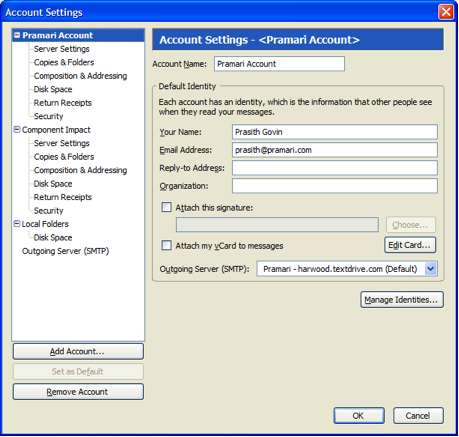
\includegraphics{thunderbird1.png}}
\caption{\label{fig:thunderbird1} Thunderbird 1}
\end{figure}

\begin{figure}
\resizebox{\textwidth}{!}{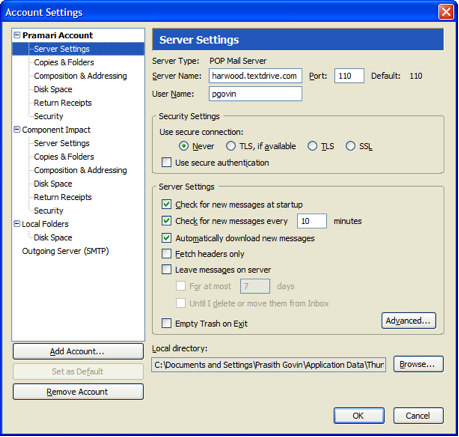
\includegraphics{thunderbird2.png}}
\caption{\label{fig:thunderbird2} Thunderbird 1}
\end{figure}

\begin{figure}
\resizebox{\textwidth}{!}{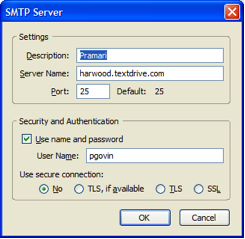
\includegraphics{thunderbird3.png}}
\caption{\label{fig:thunderbird3} Thunderbird 1}
\end{figure}

\subsection{Project Management Software}

We use Scrum to manage our development projects.  There's a plethora of Scrum tutorials, guides and books, but you can probably grok everything you need on-the-job.  That said, I recommend \cite{scrum-guide} as a brief introduction, and the original publication \cite{scrum-book} for a more thorough treatment.  We have a copy of \cite{scrum-book} in the office.

We use basecamp \cite{basecamp} for client facing project management and documentation, and we use Rally \cite{rallydev} for Sprint planning and tracking (Sprints are the units of work in Scrum).  You should have accounts to both of these, so let someone know if you do not.

\section{Development Environment}

Our development process, for better or worse, is very tightly coupled to the eclipse\cite{eclipse} platform.  If you completed Section~\ref{os}, then eclipse should be installed on your system.  From Ubuntu, click $applications->development$.  We recommend creating a workspace for each project, as depicted in Figure~\ref{fig:eclipse1}.

All RIFIDI-based software can be downloaded from our online repositories \cite{rep-edge, rep-external, rep-internal, rep-ambient}.  Subclipse \cite{subclipse} is an Eclipse plugin that we use to interface with our SVN server.  To install Subclipse, from within Eclipse click: \begin{verbatim}Help->Install new software.\end{verbatim}  Figure~\ref{fig:eclipse2} shows this.

A dialog box will appear; click on add, paste in the Subclipse update site URL \cite{subclipse-update}; see Figure~\ref{fig:eclipse3} for visual verification.  This should show you the available software.  Check all required boxes and click finish.  The Subclipse documentation is installed with the plugin, and it can be accessed from within Eclipse help.  An online version can be found at \cite{subclipse-doc}.

\begin{figure}
\resizebox{\textwidth}{!}{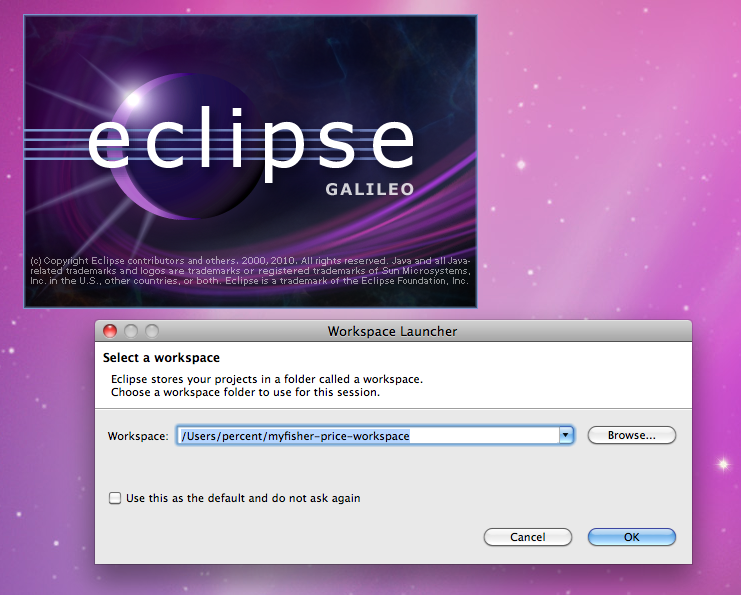
\includegraphics{eclipse1.png}}
\caption{\label{fig:eclipse1} Eclipse workspace}
\end{figure}

\begin{figure}
\resizebox{\textwidth}{!}{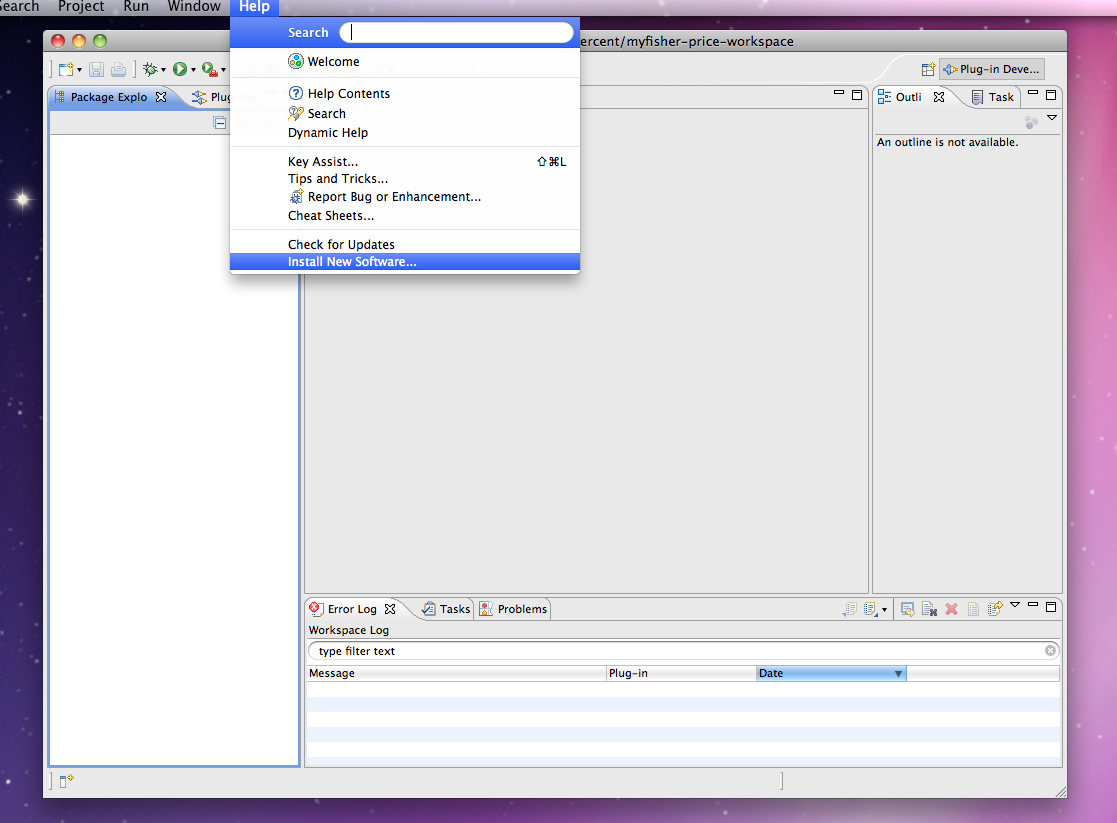
\includegraphics{eclipse2.png}}
\caption{\label{fig:eclipse2} Eclipse software installation }
\end{figure}

\begin{figure}
\resizebox{\textwidth}{!}{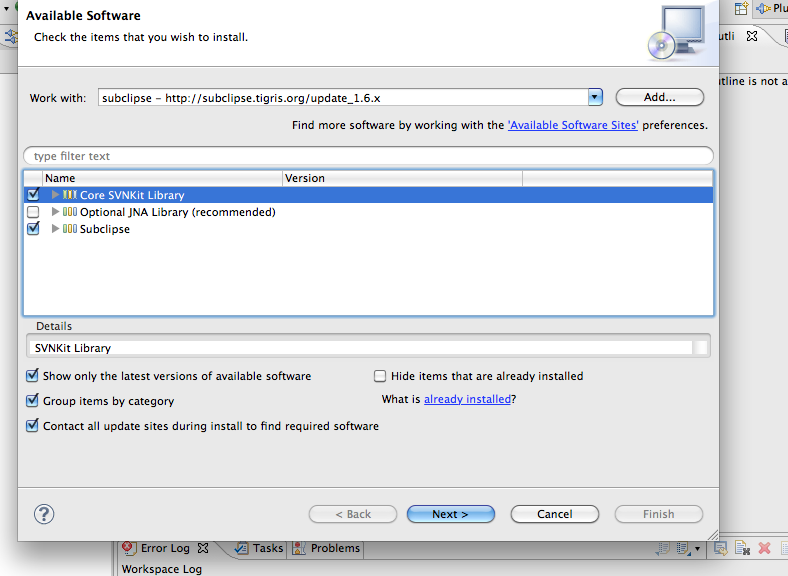
\includegraphics{eclipse3.png}}
\caption{\label{fig:eclipse3} Subclipse }
\end{figure}

\begin{figure}
\resizebox{\textwidth}{!}{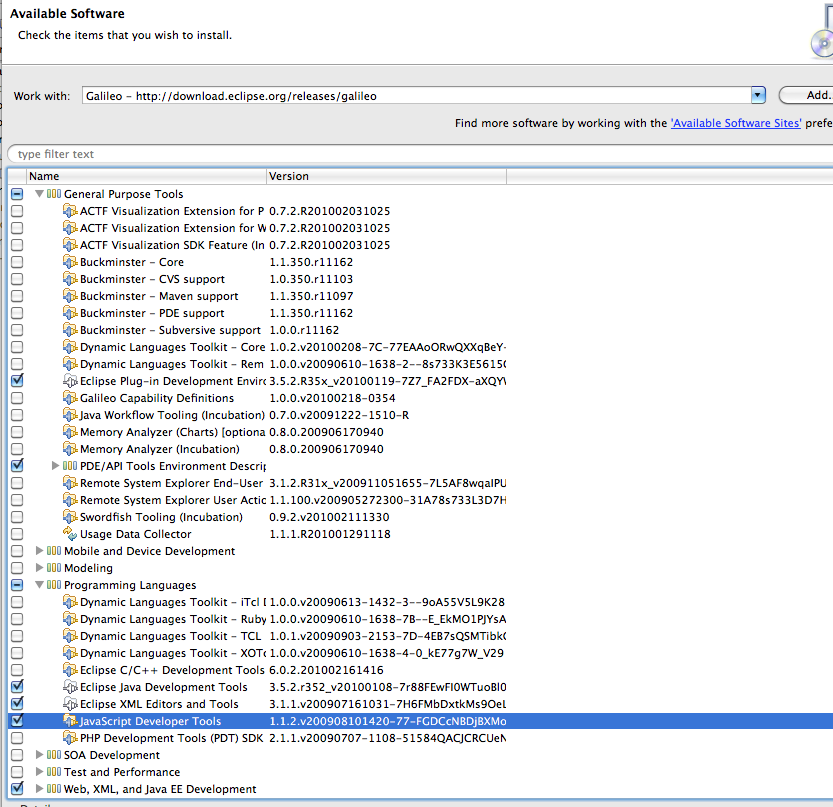
\includegraphics{eclipse4.png}}
\caption{\label{fig:eclipse4} Subclipse }
\end{figure}


\begin{figure}
\resizebox{\textwidth}{!}{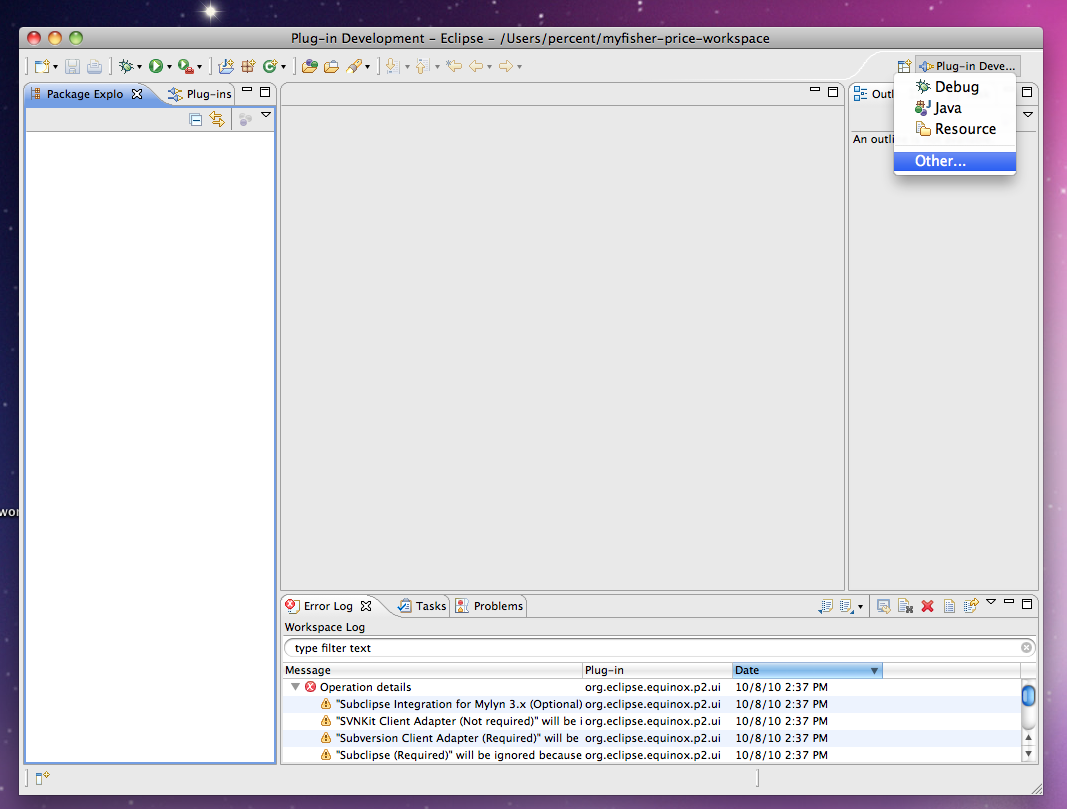
\includegraphics{eclipse5.png}}
\caption{\label{fig:eclipse5}  }
\end{figure}

\begin{figure}
\resizebox{\textwidth}{!}{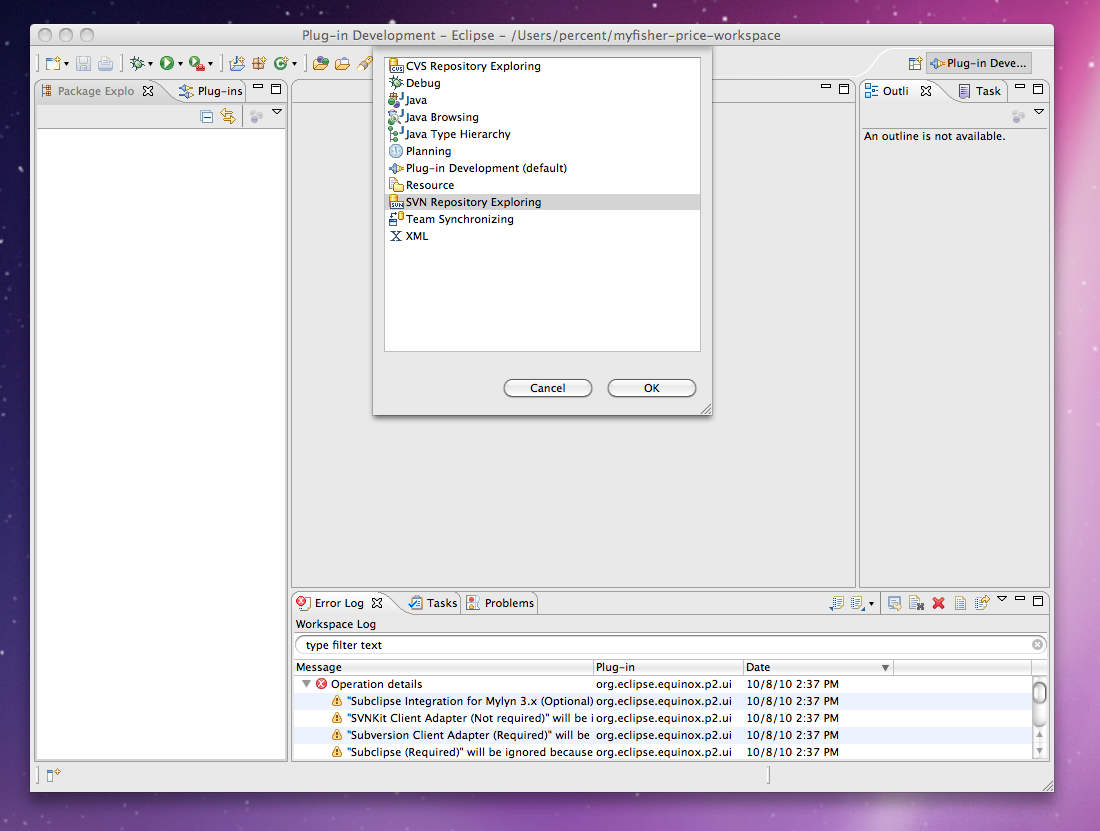
\includegraphics{eclipse6.png}}
\caption{\label{fig:eclipse6}  }
\end{figure}


\begin{figure}
\resizebox{\textwidth}{!}{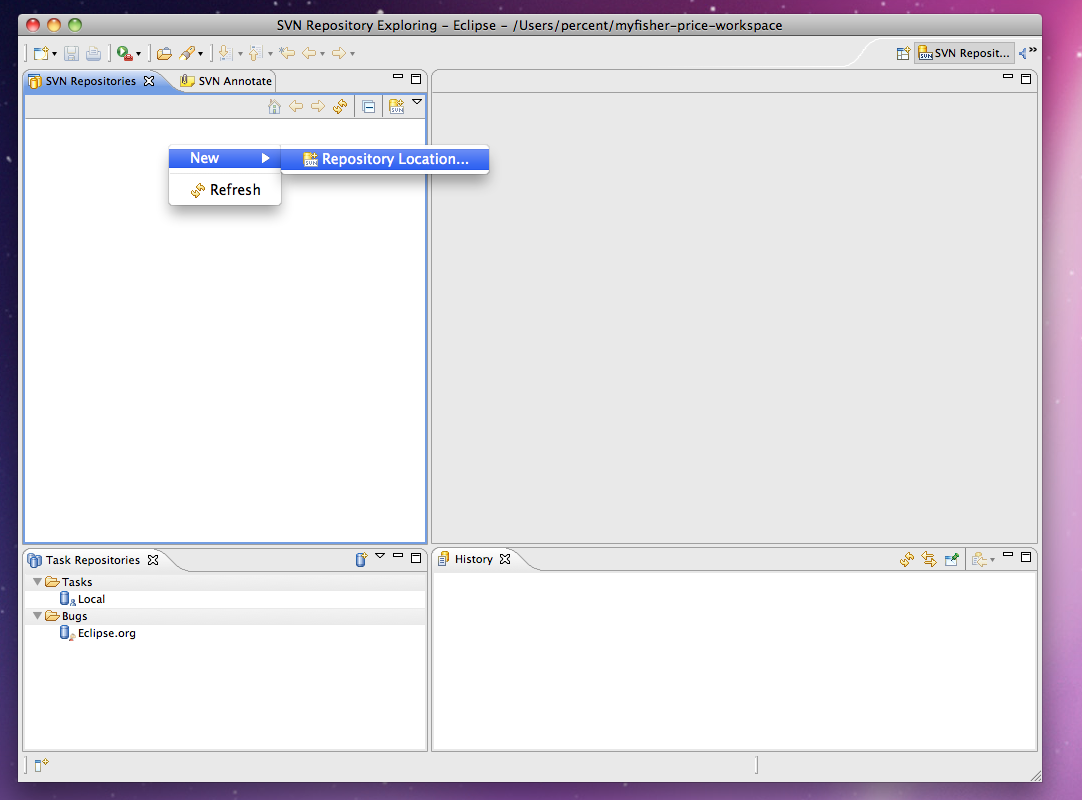
\includegraphics{eclipse7.png}}
\caption{\label{fig:eclipse7}}
\end{figure}


\begin{figure}
\resizebox{\textwidth}{!}{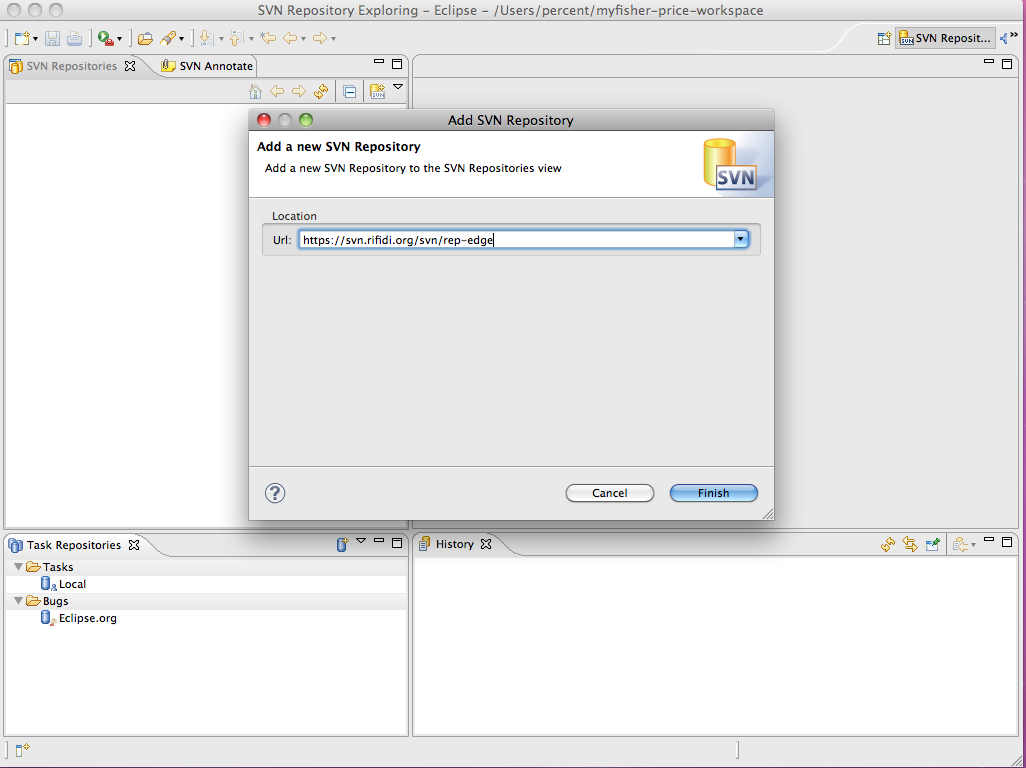
\includegraphics{eclipse8.png}}
\caption{\label{fig:eclipse8} }
\end{figure}


\begin{figure}
\resizebox{\textwidth}{!}{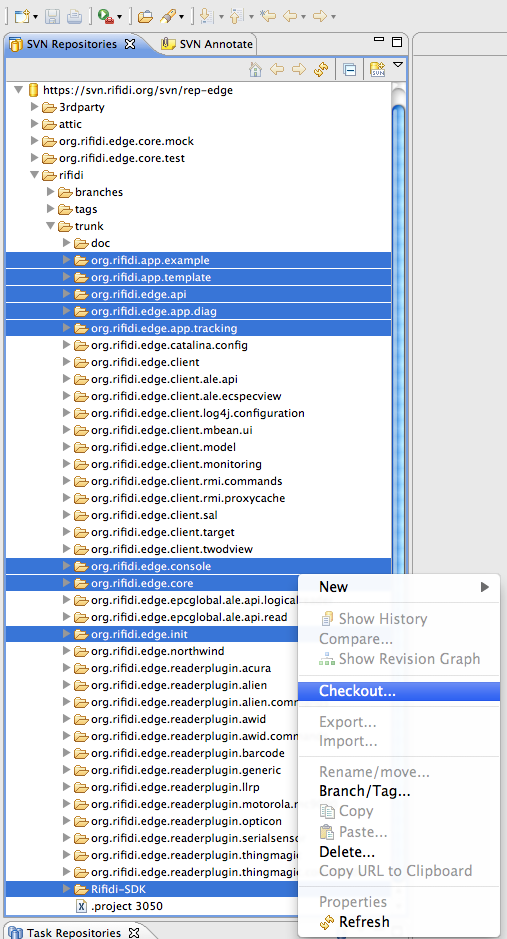
\includegraphics{eclipse9.png}}
\caption{\label{fig:eclipse9} Checking out sources }
\end{figure}

 \subsection{Edge Server}
\subsubsection{ Configuration}

First we need to create a new repository location.  From within to do this within the SVN Repository browsing view, click 
\begin{verbatim}  
File->New->SVN->Checkout projects From SVN
\end{verbatim}

Add the URL for the Edge Server repository \cite{rep-edge}.  Next we'll check out the target platform

Next click through the 


Eclipse.location from within Eclipse.  To do this go to the SVN Repository Browsing

\subsubsection{Running Unit, System and RegressionTests}
\subsubsection{Adding Platform Features}
\subsubsection{Creating Edge-Server Applications}
\subsubsection{Testing Applications}
\subsubsection{Platform Deployment}

\begin{thebibliography}{99}
\bibitem{ubuntu} Ubuntu Releases.  \url{http://releases.ubuntu.com}.
\bibitem{lucid} Ubuntu 10.04.1.  \url{http://releases.ubuntu.com/lucid}.
\bibitem{lucid-doc} Ubuntu 10.04.1 Documentation. \url{https://help.ubuntu.com/10.04/index.html}.
\bibitem{apt-get-tut} Apt.  \url{http://www.debian.org/doc/manuals/apt-howto/ch-apt-get.en.html}.
\bibitem{basecamp} Pramari Basecamp.  \url{https://pramari.basecamphq.com}.
\bibitem{rallydev}  Rally.  \url{https://community.rallydev.com}.
\bibitem{scrum-book}  Schwaber, Ken. Agile Project Management with Scrum.
\bibitem{scrum-guide} Scrum Guide.  \url{http://www.scrum.org/scrumguideenglish}. 
\bibitem{rep-edge} RIFIDI Edge Server. \url{https://svn.rifidi.org/svn/rep-edge}.
\bibitem{rep-external} RIFIDI Toolkit. \url{https://svn.rifidi.org/svn/rep-external}.
\bibitem{rep-internal} RIFIDI ?? . \url{https://svn.rifidi.org/svn/rep-internal}.
\bibitem{rep-ambient} Ambient Project. \url{https://svn.rifidi.org/svn/rep-ambient}.
\bibitem{eclipse} Eclipse.  \url{http://www.eclipse.org.}.
\bibitem{subclipse} Subclipse.  \url{http://subclipse.tigris.org/}.
\bibitem{subclipse-doc} Subclipse online documentation.  \url{http://svn.collab.net/subclipse/help/index.jsp}
\bibitem{subclipse-update} Subclipse.  \url{http://subclipse.tigris.org/update_1.6.x}
\end{thebibliography}
\end{document}  


